\let\textcircled=\pgftextcircled
\chapter{Feasibility Study}
\section{Define The Problem}

Currently, businesses globally have to communicate across multiple departments and management systems to facilitate cross-company transactions, leading to costly mistakes, opaque interaction histories, high administration costs and long delays for the transference of capital to be processed. Business blockchains, an innovative solution to this global issue, are reinventing how transactions are managed. They can take time and costs out of almost any process, enabling near real-time operations. And they deliver a high degree of accuracy and control, with much less risk than many alternatives. Due to the immutable nature of the blockchain, a transparent record of all transactions is kept which can be utilised for bookkeeping and taxation purposes while also preventing fraudulent behaviour as all transactions are recorded and can be reproduced for litigious reasons. The business blockchain that is being created, therefore, will help supply chain partners and corporations globally by creating a complete, transparent, tamperproof history and facilitation of the information flows, inventory flows, and financial flows in transactions. This permissioned blockchain will outperform current enterprise resource planning solutions as it is able to manage all transactions extremely quickly and efficiently, through sharing the load of computation across all nodes in the blockchain. An example of the differences between conventional record keeping and blockchain for a transaction is shown below. \\

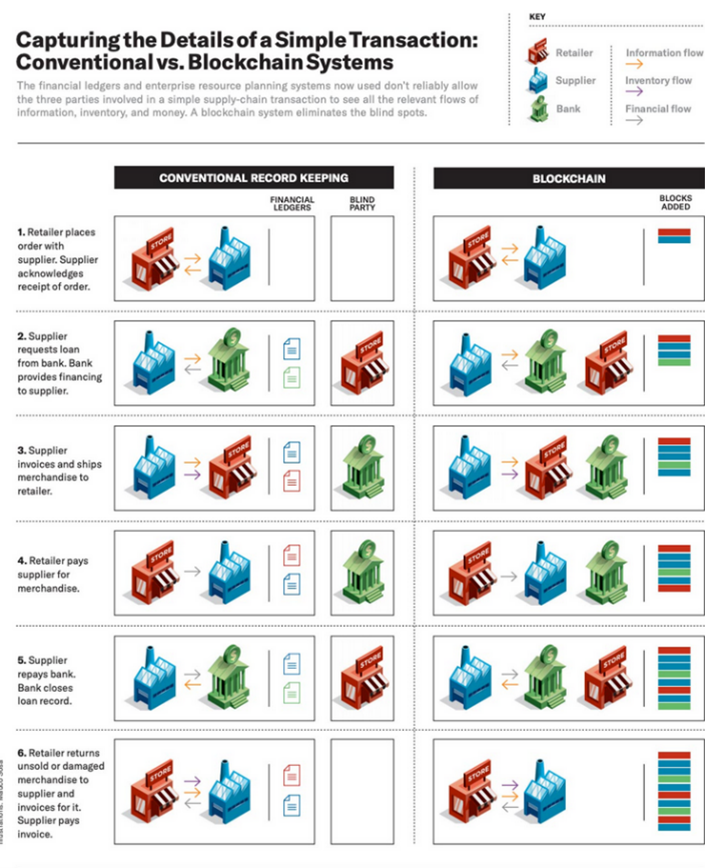
\includegraphics[width=\linewidth]{figures/vs.png} \\

The blockchain that is being developed is a proof of concept that will show the core functionality of permissioned blockchains and the benefits it produces. It will be compatible for all businesses as a node will be able to run on a server setup by the development team and users can interface with the system via a user-friendly web frontend to manage transactions and assets. The assets, labour and even items such as orders / invoices within each company will be tokenised on the blockchain so that businesses can interact with other businesses over the blockchain. Though it most commonly refers to the tokenization of financial or fungible assets, such as shares in a company or a quantity of gold, asset tokenization can hypothetically refer to the tokenization of any material or nonmaterial thing possessing monetary value: everything from a piece of art to a patent to an hour of a skilled worker’s time. This process of tokenization creates a bridge between real-world assets and their trading, storage and transfer in a digital world.\\

Although the functionality of transferring fungible and non-fungible assets will be implemented into the software solution, the legal processes surrounding the binding of assets will be implemented in the future. These legal proceedings are outside the scope of this project as they would require communication with governing institutions, intricate understanding of taxation law and connecting software solutions with the strenuous obligations of regulatory frameworks. \\

For the purpose of this conceptual design, I will utilise a main, “converge” token that is not truly backed by US Dollar or another asset, but in production, would be. The manner in which the tokens will be bound to physical assets is through the creation of a stable coin which reassures businesses will not have to consider the fluctuations of token value. To make this collateralised stable coin I would need to own the fiat or assets in which the token was based upon, as ‘collateral’ or conduct an exchange agreement with a bank in which the converge tokens could be converted into the local fiat currency. \\

\section{Economic Feasibility}
The economic feasibility of this project can be understood through a number of points of analysis. Firstly, the spending projection of the project needs to be addressed and how much working capital is required for the functioning of the software. Secondly, the cash flows need to be examined, including the revenues and the maintaining outflows of cash. \\

The spending projection for this project needs to be minimal as this scope of this project does not enable me to spend capital on expensive APIs, or high-end virtual private servers to host nodes for testing and compatibility studies. Thus, I have planned the project to use the most minimal costs possible as this fits within the boundaries of the project. I have utilised open-source frameworks to reduce costs and cut out any dependence on APIs. If this project was to be produced in reality, I would need to set aside ‘collateral’ in which the converge token was tied to so that it had a physical asset that it was bound to. This would be quite economically infeasible so a better method would be to conduct an exchange agreement with a bank in which the converge tokens could be converted into the local fiat currency. \\

The projected income expected from this project will come in the form of small fees that are collected on each transaction, although a small percentage, the sheer volume will make the process very economically advantageous. For example, a percentage for transaction such as 0.1\% will be a large incentive for continuing development and maintenance as if a trillion dollars passes through the network, that is around one billion dollars in revenue. If large volumes of transaction are occurring every day, then this will lead to a high profit. Further, as there are no central servers, the maintenance cost of the blockchain will be quite minimal, leading to lower expenditure and thus higher profits.

\section{Technical Feasibility}

Technical feasibility is the process of figuring out how you are going to produce your product or service to determine whether it is possible to create. Thus, with the aid of thorough research the software solution is feasible to create, however, it would require quite sophisticated technology that is only currently being developed. Firms around the globe are all attempting to understand and implement blockchain technology into their business, which reveals the pioneering needed to develop and implement such a software solution. Although it is technically feasible to create, the difficulty of creating will be high. Due to access to blockchain frameworks such as substrate, however, the ease of creating such a software is increased.\\

\section{Operational Feasibility}

Operational feasibility is the measure of how well a proposed system solves the problems and takes advantage of the opportunities identified during the problem definition. The software solution that is being proposed will reduce costly mistakes through the utilisation of smart contracts and sophisticated consensus mechanisms, reduce the often-unintelligible transaction histories, and reduce long delays for the transference of assets through sophisticated networking protocols. \\

The software solution will be a proof of concept / prototype of a fully functioning business blockchain; thus, it will not be able to be utilised by business's globally. This slightly lowers its operational feasibility, however, if successful in demonstrating the capabilities of a business blockchain then further development would be more greatly supported. The software solution will be able to be operationally feasible as its design, although complex and requiring meticulous pre-thought, is manageable. In conjunction, the maintainability of the software solution is quite high as, inherent to blockchain technology, servers are not needed due to its distributed nature. Through forkless runtime upgrades, the system can be updated and maintained without the need for it to ever be stopped, aiding to the unbeatable uptime. The hard part of this project in reality is establishing a sustainable group of trading partners, with transactions governed by effective smart contracts and clear rules of engagement. \\

\section{Scheduling Feasibility}

Schedule Feasibility is defined as the probability of a project to be completed within its scheduled time limits, by a planned due date. In comparison to the scale of this project, the timeframe that has been allocated is quite limited. The total time to design, develop, produce and test the software solution is 60 days. This does make completion of the project difficult and does introduce a few scheduling issues into the analysis of the feasibility. To solve this, scheduling tools such as Gantt charts will optimise workflows and time management, enabling development to be at its maximum efficiency. Although there is a very restrictive timeframe, the project is still feasible as long as time is effectively managed. \\

\section{Recommendation}

Due to each individual aspect of the feasibility report revealing an advantageous position in creating the software, the recommendation is to develop the software solution. This recommendation is based off the high results from each section; however, it will be acknowledged that the production of the software in the timeframe will be quite challenging, due to the sheer magnitude of the software solution proposed. \\



